\chapter{Synthese: rendement en zuiverheid}\label{ch:g10:synthesis-yield}

Aspirine is een van de meest gebruikte geneesmiddelen ter wereld. Het
verhaal begint bij wilgenbast, waarop lang gekauwd werd tegen pijn en
koorts; de werkzame stof van de bast werd in de negentiende eeuw
herleid tot een familie verbindingen waaruit scheikundigen salicylzuur
maakten. Salicylzuur was te hard voor de maag om in grote doses in te
nemen, en werd omgezet in een mildere stof, acetylsalicylzuur: aspirine.
Tegenwoordig wordt het per ton gemaakt in stalen reactoren, met dezelfde
reactie die een schoollaboratorium in een middag kan uitvoeren. Een stof
maken is maar de helft van het werk: ze moet ook gescheiden worden van
al het andere in de kolf, gezuiverd, gecontroleerd en gewogen, om te
zien hoeveel van wat mogelijk was er echt verkregen is.

\begin{recall}
\omterm{def:g10:chemical-species:extraction}{Extractie}, \omterm{def:g10:chemical-species:distillation}{destillatie}, \omterm{def:g10:chemical-species:tlc}{dunnelaagchromatografie} en de \omterm{def:g10:chemical-species:retention-factor}{retentiefactor};
een zuivere vaste stof smelt scherp bij een bekende temperatuur
(\cref{ch:g10:chemical-species}). Een filter houdt een vaste stof tegen
en laat een vloeistof door (\cref{ch:g3:separating-mixtures}). De
\omterm{def:g10:reaction-progress-table:extent}{voortgangstabel} geeft de maximale hoeveelheid product uit de \omterm{def:g10:reaction-progress-table:limiting}{beperkende
beginstof} (\cref{ch:g10:reaction-progress-table}).
\end{recall}

\begin{omfigure}
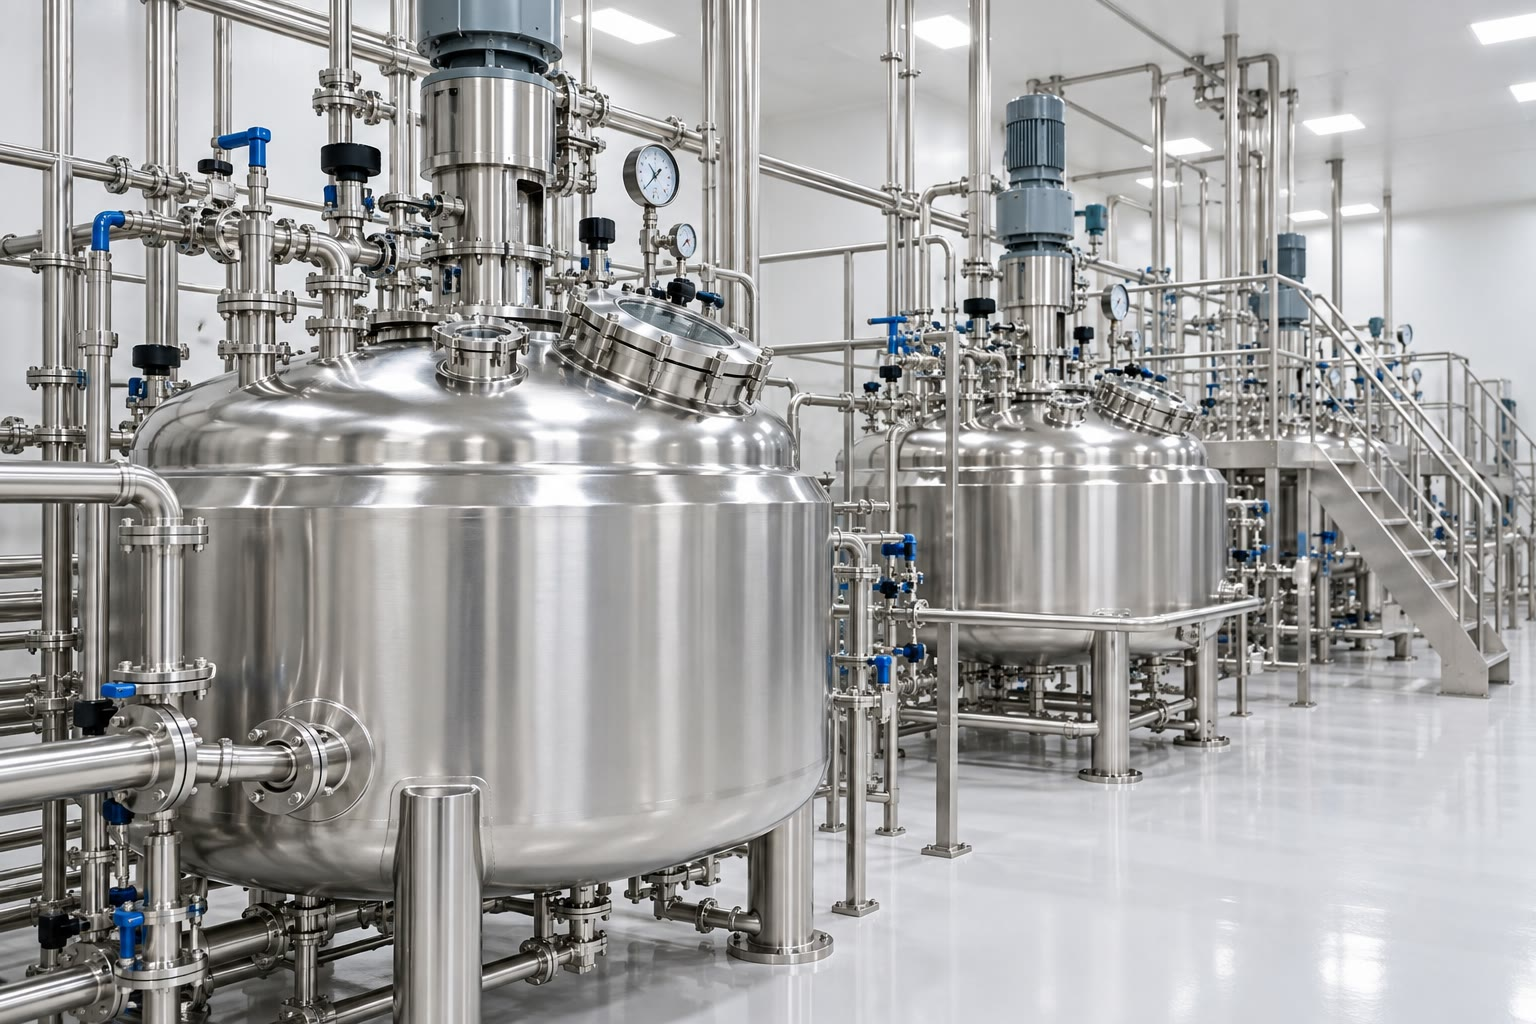
\includegraphics[width=0.55\linewidth]{images/book1/ai/g10-pharma-reactor.jpg}

{\small Stalen reactoren in een farmaceutische fabriek: een \omterm{def:g10:synthesis-yield:synthesis}{synthese} uit
het laboratorium, een miljoen keer opgeschaald.}
\end{omfigure}

\section{De stappen van een synthese}

\begin{definition}[Synthese, ruw product]\label{def:g10:synthesis-yield:synthesis}
Een \emph{synthese}\index{synthese} is het maken van een \omterm{def:g6:pure-substances-and-mixtures:species}{chemische stof}
met een of meer \omterm{def:g7:chemical-reactions:reaction}{chemische reacties}, uitgaande van andere stoffen. De
vaste stof of vloeistof die je rechtstreeks uit het reactiemengsel
haalt, vóór enige zuivering, is het \emph{ruwe product}\index{ruw product}:
het bevat nog \omterm{def:g7:chemical-reactions:reactant}{beginstoffen}, bijproducten en \omterm{def:g6:solutions-and-solubility:solute}{oplosmiddel}.
\end{definition}

\begin{method}[Een synthese plannen]\label{met:g10:synthesis-yield:plan}
Een \omterm{def:g10:synthesis-yield:synthesis}{synthese} verloopt in vier stappen:
\begin{enumerate}
  \item \textbf{Reactie}: meng de \omterm{def:g7:chemical-reactions:reactant}{beginstoffen} in de juiste hoeveelheden,
        vaak met één ervan in overmaat, en verwarm zo nodig.
  \item \textbf{Isolatie}: scheid het \omterm{def:g10:synthesis-yield:synthesis}{ruwe product} van het reactiemengsel
        (filtratie, \omterm{def:g10:chemical-species:extraction}{extractie}).
  \item \textbf{Zuivering}: verwijder de verontreinigingen uit het \omterm{def:g10:synthesis-yield:synthesis}{ruwe
        product} (\omterm{def:g10:synthesis-yield:recrystallisation}{herkristallisatie} voor een vaste stof, \omterm{def:g10:chemical-species:distillation}{destillatie} voor
        een vloeistof).
  \item \textbf{Analyse}: controleer de identiteit en de zuiverheid van
        het product (smeltpunt, chromatografie), weeg het en bereken het
        \omterm{def:g10:synthesis-yield:yield}{rendement}.
\end{enumerate}
\end{method}

\begin{example}[Aspirine maken]\label{ex:g10:synthesis-yield:aspirin}
Salicylzuur reageert met ethaanzuuranhydride (ook azijnzuuranhydride
genoemd) tot aspirine en ethaanzuur:
\[
  \ce{C7H6O3 + C4H6O3 -> C9H8O4 + C2H4O2}
\]
\[
  \text{salicylzuur} + \text{ethaanzuuranhydride} \longrightarrow
  \text{aspirine} + \text{ethaanzuur}.
\]
Het anhydride wordt in overmaat toegevoegd, zodat al het salicylzuur
reageert; het ethaanzuur dat ontstaat, is een bijproduct.
\end{example}

\begin{omfigure}
\setchemfig{atom sep=1.7em}
\begin{tabular}{@{}c@{\enspace}c@{\enspace}c@{\enspace}c@{\enspace}c@{\enspace}c@{\enspace}c@{}}
\chemfig{*6(-=-(-COOH)=(-OH)-=)} & $+$ &
\chemfig{H_3C-C(=[2]O)-O-C(=[2]O)-CH_3} & $\longrightarrow$ &
\chemfig{*6(-=-(-COOH)=(-O-[:150]C(=[:90]O)-[:210]H_3C)-=)} & $+$ &
\chemfig{H_3C-C(=[2]O)-OH} \\[2pt]
\small salicylzuur & & \small ethaanzuuranhydride & &
\small aspirine & & \small ethaanzuur
\end{tabular}\par\medskip

{\small Het maken van aspirine, in getekende formules (elk hoekpunt van
de zeshoek is een koolstofatoom, met een waterstofatoom waar niets anders
getekend is; een later hoofdstuk legt deze verkorte schrijfwijze uit). De
\ce{-OH}-groep op de ring van salicylzuur neemt de helft van het
anhydride op; de andere helft vertrekt als ethaanzuur.}
\end{omfigure}

\section{Verwarmen onder terugvloeiing}

\begin{definition}[Verwarmen onder terugvloeiing]\label{def:g10:synthesis-yield:reflux}
\emph{Verwarmen onder terugvloeiing}\index{verwarmen onder terugvloeiing}
is een reactiemengsel verwarmen in een kolf met daarop een verticale
koeler: de dampen stijgen op, koelen af in de koeler, en de vloeistof
stroomt terug in de kolf.
\end{definition}

\begin{proposition}[Waarom terugvloeiing]\label{prop:g10:synthesis-yield:why-reflux}
Verwarmen maakt de meeste reacties sneller; terugvloeiing maakt het
mogelijk zo lang als nodig te verwarmen bij het kookpunt van het
\omterm{def:g6:pure-substances-and-mixtures:mixture}{mengsel}, zonder dat er \omterm{def:g7:chemical-reactions:reactant}{beginstof}, product of \omterm{def:g6:solutions-and-solubility:solute}{oplosmiddel} als damp
verloren gaat.
\end{proposition}

\begin{proof}
De temperatuur van een kokende vloeistof kan niet boven haar kookpunt
stijgen, en alle damp die uit de vloeistof ontsnapt, wordt gecondenseerd
en teruggevoerd: er verlaat niets de opstelling, die bovenaan open blijft
zodat er geen druk ontstaat.
\end{proof}

\begin{omfigure}
\begin{tikzpicture}[font=\small, scale=1.05]
  \pic[transform shape] at (0,0) {heatingmantle};
  \pic[transform shape] at (0,0) {rbflask={0.42}{orange!25}};
  \foreach \p in {(-0.3,0.25), (0.2,0.18), (0.45,0.4), (-0.5,0.5)}
    \fill[black!45] \p circle (0.05);
  \pic[transform shape] at (0,3.0) {condenser};
  \draw[omDef, thick, <-] (0.8,3.825) -- (1.9,3.825) node[right] {water in};
  \draw[omDef, thick, ->] (0.8,5.375) -- (1.9,5.375) node[right] {water uit};
  \draw[omProp, thick, <-] (-0.18,5.8) -- (-1.4,6.1) node[left] {open bovenkant};
  \draw[omProp, thick, <-] (-0.45,1.2) -- (-2.0,1.6)
    node[left, align=right] {reactiemengsel\\ en kooksteentjes};
  \draw[omProp, thick, <-] (-1.35,-0.2) -- (-2.0,-0.6)
    node[left] {verwarmingsmantel};
  \draw[omThm, ->, thick] (-0.05,3.4) -- (-0.05,4.3);
  \draw[omDef, ->, thick] (0.05,4.3) -- (0.05,3.4);
  \node[omThm, anchor=east, font=\footnotesize] at (-0.45,4.6) {damp stijgt op};
  \node[omDef, anchor=west, font=\footnotesize] at (0.85,4.6) {vloeistof valt terug};
\end{tikzpicture}

{\small \omterm{def:g10:synthesis-yield:reflux}{Verwarmen onder terugvloeiing}. Koud water komt onderaan de mantel
van de koeler binnen en gaat er bovenaan uit, zodat de mantel altijd vol
is.}
\end{omfigure}

\begin{remark}[Water onderaan erin]\label{rem:g10:synthesis-yield:water}
Komt het water van boven, dan loopt het meteen naar beneden en blijft
het bovenste deel van de mantel met \omterm{def:g4:air-a-mixture-of-gases:air}{lucht} gevuld; komt het van onderen,
dan moet het de hele mantel vullen voordat het eruit kan.
\end{remark}

\section{Isoleren en zuiveren}

\begin{definition}[Vacuümfiltratie]\label{def:g10:synthesis-yield:vacuum-filtration}
\emph{Vacuümfiltratie}\index{vacuümfiltratie} is een filtratie waarbij de
vloeistof door zuiging door het filtreerpapier getrokken wordt: een
platte trechter met een geperforeerde plaat (een büchnertrechter) staat
op een afzuigkolf die op een vacuümpomp is aangesloten.
\end{definition}

\begin{omfigure}
\begin{tikzpicture}[font=\small, scale=1.05]
  \pic[transform shape] (ff) at (0,0) {filterflask={0.12}{orange!20}};
  \fill[black!50] (-0.3,2.45) rectangle (0.3,2.8);
  \pic[transform shape] at (0,2.45) {buchner={black!8}};
  \draw[black!60, line width=2pt] (ff-arm) -- (2.6,2.2);
  \draw[omProp, thick, ->] (2.7,2.2) -- (3.4,2.2) node[right,
    align=left, text=black] {naar de\\ vacuümpomp};
  \draw[omProp, thick, <-] (0.7,3.8) -- (1.9,4.3) node[right, text=black]
    {kristallen op filtreerpapier};
  \draw[omProp, thick, <-] (-0.4,0.15) -- (-1.8,0.6) node[left, text=black]
    {filtraat};
  \draw[omProp, thick, <-] (-0.3,2.6) -- (-1.8,2.9) node[left, text=black]
    {rubberen ring};
\end{tikzpicture}

{\small \omterm{def:g10:synthesis-yield:vacuum-filtration}{Vacuümfiltratie} met een büchnertrechter: de pomp trekt de
vloeistof er snel doorheen en laat de vaste stof bijna droog achter.}
\end{omfigure}

\begin{definition}[Herkristallisatie]\label{def:g10:synthesis-yield:recrystallisation}
\emph{Herkristallisatie}\index{herkristallisatie} zuivert een vaste stof
door haar op te lossen in een zo klein mogelijk volume heet
\omterm{def:g6:solutions-and-solubility:solute}{oplosmiddel} en de oplossing dan te laten afkoelen: het product, dat koud
veel minder oplosbaar is, kristalliseert uit, terwijl de
verontreinigingen, die in kleine hoeveelheden aanwezig zijn, opgelost
blijven.
\end{definition}

\begin{method}[Een vaste stof herkristalliseren]\label{met:g10:synthesis-yield:recrystallise}
\begin{enumerate}
  \item Kies een \omterm{def:g6:solutions-and-solubility:solute}{oplosmiddel} waarin het product heet heel goed en koud
        nauwelijks \omterm{def:g2:mixing-and-dissolving:dissolve}{oplost}.
  \item Voeg het hete \omterm{def:g6:solutions-and-solubility:solute}{oplosmiddel} beetje bij beetje toe aan de ruwe
        vaste stof, net tot alles is opgelost.
  \item Laat de oplossing langzaam afkoelen, daarna in een ijsbad: er
        ontstaan kristallen.
  \item Verzamel ze met \omterm{def:g10:synthesis-yield:vacuum-filtration}{vacuümfiltratie}, was ze met een beetje ijskoud
        \omterm{def:g6:solutions-and-solubility:solute}{oplosmiddel} en droog ze.
\end{enumerate}
\end{method}


\begin{omfigure}
\begin{tikzpicture}[font=\small]
  % 1. crude solid + a little hot solvent, on a hot plate
  \pic at (0,0.3) {hotplate};
  \pic at (0,0.3) {erlenmeyer={0.18}{orange!12}};
  \foreach \p in {(-0.4,0.42),(-0.15,0.38),(0.1,0.45),(0.35,0.4),(-0.3,0.55),(0.2,0.6)}
    \fill[brown!60] \p circle (0.06);
  \node[align=center, anchor=north] at (0,-0.15) {1. ruwe vaste\\ stof, heet\\ oplosmiddel};
  % 2. clear hot solution
  \pic at (3,0.3) {hotplate};
  \pic at (3,0.3) {erlenmeyer={0.22}{orange!12}};
  \node[align=center, anchor=north] at (3,-0.15) {2. alles\\ opgelost, helder\\ en heet};
  % 3. ice bath: crystals
  \fill[cyan!12, draw=black!40] (5.0,0) rectangle (7.0,1.2);
  \foreach \p in {(5.2,0.9),(6.75,1.0),(5.3,0.3),(6.8,0.25)}
    \draw[black!35, fill=white] \p ++(-0.12,-0.1) rectangle ++(0.24,0.2);
  \pic at (6,0.1) {erlenmeyer={0.2}{orange!8}};
  \foreach \x/\y in {-0.45/0.18,-0.25/0.15,0/0.2,0.25/0.15,0.45/0.2,-0.1/0.3,0.15/0.32,
                     -0.35/0.32,0.35/0.33}
    \fill[white, draw=black!55] (6+\x,0.1+\y) -- ++(0.07,0.06) -- ++(0.07,-0.06)
      -- ++(-0.07,-0.06) -- cycle;
  \node[align=center, anchor=north] at (6,-0.15) {3. afkoelen\\ in ijs:\\ kristallen};
  % 4. filter
  \pic at (9,0) {filterflask={0.12}{orange!12}};
  \pic at (9,2.45) {buchner={black!12}};
  \fill[black!50] (8.7,2.45) rectangle (9.3,2.8);
  \node[align=center, anchor=north] at (9,-0.15) {4. vacuüm-\\ filtreren, koud\\ wassen, drogen};
\end{tikzpicture}

{\small \omterm{def:g10:synthesis-yield:recrystallisation}{Herkristallisatie} in vier stappen. De verontreinigingen blijven
opgelost in het koude \omterm{def:g6:solutions-and-solubility:solute}{oplosmiddel} en gaan mee in het \omterm{def:g3:separating-mixtures:filter}{filtraat}.}
\end{omfigure}

\begin{remark}[Verliezen zijn onvermijdelijk]\label{rem:g10:synthesis-yield:losses}
% ledger: sol:aspirin-25, sol:aspirin-37
Ook koud houdt het \omterm{def:g6:solutions-and-solubility:solute}{oplosmiddel} wat product opgelost. Aspirine lost in
water op tot ongeveer \qty{3.3}{g/L} bij \qty{25}{\celsius}, drie keer
zoveel bij \qty{37}{\celsius}, en veel meer als het heter is: elke
milliliter \omterm{def:g3:separating-mixtures:filter}{filtraat} en waswater neemt een beetje aspirine mee. Een
\omterm{def:g10:synthesis-yield:recrystallisation}{herkristallisatie} koopt zuiverheid ten koste van massa.
\end{remark}

\section{Het product analyseren}

\begin{proposition}[Twee zuiverheidscontroles]\label{prop:g10:synthesis-yield:checks}
Een gesynthetiseerde vaste stof is zuiver, binnen de grenzen van deze
tests, als:
\begin{itemize}
  \item ze scherp smelt bij het smeltpunt uit de tabellen;
  \item ze op een DLC-plaatje één enkele vlek geeft, op dezelfde hoogte
        als een monster van de \omterm{def:g6:pure-substances-and-mixtures:pure-substance}{zuivere stof}.
\end{itemize}
\end{proposition}

\begin{proof}
Aangenomen: een verontreiniging verlaagt het smeltpunt en spreidt het
over een traject (\cref{ch:g10:chemical-species}), en een tweede stof
legt op het plaatje meestal een andere afstand af.
\end{proof}

\begin{omfigure}
\begin{tikzpicture}[font=\small, scale=1.3]
  \pic[transform shape] at (0,0) {tlcplate};
  \draw[black!50, dashed] (-0.7,2.7) -- (0.7,2.7);
  % lanes: C crude, R recrystallised, A aspirin, S salicylic acid
  \foreach \x/\l in {-0.5/C,-0.17/R,0.17/A,0.5/S}
    \node[font=\footnotesize, anchor=north] at (\x,0.38) {\l};
  \fill[omDef!70] (-0.5,1.75) ellipse (0.09 and 0.06);
  \fill[omDef!40] (-0.5,1.25) ellipse (0.09 and 0.06);
  \fill[omDef!70] (-0.17,1.75) ellipse (0.09 and 0.06);
  \fill[omDef!70] (0.17,1.75) ellipse (0.09 and 0.06);
  \fill[omDef!70] (0.5,1.25) ellipse (0.09 and 0.06);
  \node[anchor=west, font=\footnotesize] at (0.85,2.7) {front van het eluens};
  \node[anchor=west, font=\footnotesize] at (0.85,0.4) {startlijn};
\end{tikzpicture}

{\small Chromatografie van het \omterm{def:g10:synthesis-yield:synthesis}{ruwe product} (C) en het geherkristalliseerde
product (R) naast zuivere aspirine (A) en salicylzuur (S), bekeken onder
ultraviolet licht. Het \omterm{def:g10:synthesis-yield:synthesis}{ruwe product} bevat nog salicylzuur; het
geherkristalliseerde niet.}
\end{omfigure}

\section{Rendement}

\begin{definition}[Rendement]\label{def:g10:synthesis-yield:yield}
Het \emph{rendement}\index{rendement} $\eta$ van een \omterm{def:g10:synthesis-yield:synthesis}{synthese} is de
verhouding tussen de hoeveelheid product die echt verkregen is, zuiver en
droog, en de maximale hoeveelheid die de \omterm{def:g10:reaction-progress-table:limiting}{beperkende beginstof} kon geven:
\[
  \eta = \frac{n_{\text{verkregen}}}{n_{\max}} ,
\]
meestal gegeven als percentage.
\end{definition}

\begin{proposition}[Rendement uit massa's]\label{prop:g10:synthesis-yield:masses}
Omdat de verkregen en de maximale hoeveelheid over hetzelfde product
gaan, met \omterm{def:g10:the-mole:molar-mass}{molaire massa} $M$, is het \omterm{def:g10:synthesis-yield:yield}{rendement} ook de verhouding van de
massa's:
\[
  \eta = \frac{m_{\text{verkregen}}}{m_{\max}},
  \qquad m_{\max} = n_{\max} \times M,
\]
waarbij $n_{\max}$ uit de \omterm{def:g10:reaction-progress-table:extent}{voortgangstabel} komt, bij $x = x_{\max}$.
\end{proposition}

\begin{proof}
$m_{\text{verkregen}} / m_{\max} = (n_{\text{verkregen}} M) / (n_{\max} M)
= n_{\text{verkregen}} / n_{\max}$.
\end{proof}

\begin{example}[Rendement van een kleine synthese]\label{ex:g10:synthesis-yield:small}
% ledger: aw:C, aw:H, aw:O
Er reageert \qty{1.38}{g} salicylzuur ($M = \qty{138.0}{g/mol}$), dat is
\qty{0.0100}{mol}, met ethaanzuuranhydride in overmaat. De maximale
hoeveelheid aspirine is \qty{0.0100}{mol}, dat is
$0.0100 \times 180.0 = \qty{1.80}{g}$. Als er \qty{1.35}{g} zuivere,
droge aspirine verkregen wordt, is $\eta = 1.35 / 1.80 = 0.75$, een
\omterm{def:g10:synthesis-yield:yield}{rendement} van \qty{75}{\percent}.
\end{example}

\begin{remark}[Waarom rendementen onder de 100 \% liggen]\label{rem:g10:synthesis-yield:below}
Bij elke stap gaat product verloren: het blijft aan glaswerk plakken,
\omterm{def:g2:mixing-and-dissolving:dissolve}{lost op} in het \omterm{def:g3:separating-mixtures:filter}{filtraat} en het waswater, blijft achter bij een
\omterm{def:g10:synthesis-yield:recrystallisation}{herkristallisatie}; sommige reacties geven ook nevenproducten, of stoppen
voordat de \omterm{def:g10:reaction-progress-table:limiting}{beperkende beginstof} op is. Een \omterm{def:g10:synthesis-yield:yield}{rendement} boven
\qty{100}{\percent} wijst altijd op een fout, meestal een product dat
nog nat of onzuiver gewogen is.
\end{remark}

\begin{inthelab}[Aspirine maken]
In een droge kolf \omterm{def:g2:mixing-and-dissolving:mix}{mengt} de docent salicylzuur met een overmaat
ethaanzuuranhydride en een paar druppels van een zuur dat de reactie
versnelt, en verwarmt het \omterm{def:g6:pure-substances-and-mixtures:mixture}{mengsel} een kwartier onder terugvloeiing in
een waterbad van ongeveer \qty{80}{\celsius}. Na het afkoelen wordt er
koud water toegevoegd: het overtollige anhydride reageert daarmee, en de
aspirine, die nauwelijks \omterm{def:g2:mixing-and-dissolving:dissolve}{oplost} in koud water, komt eruit als witte
kristallen. Die worden met \omterm{def:g10:synthesis-yield:vacuum-filtration}{vacuümfiltratie} verzameld, geherkristalliseerd,
gedroogd en gewogen, en hun smeltpunt wordt gemeten.
\end{inthelab}

\begin{safety}{\ghs[0.82cm]{GHS02}\ghs[0.82cm]{GHS05}\ghs[0.82cm]{GHS06}\ghs[0.82cm]{GHS07}}
% ledger: ghs:acetic-anhydride, ghs:salicylic, ghs:aspirin
Ethaanzuuranhydride is ontvlambaar, schadelijk bij inslikken of
inademing, en veroorzaakt ernstige brandwonden aan huid en ogen: de
docent hanteert het in een zuurkast, met handschoenen en
veiligheidsbril. Salicylzuur is schadelijk bij inslikken en kan de ogen
beschadigen. Aspirine die in een laboratorium gemaakt is, wordt nooit als
geneesmiddel ingenomen.
\end{safety}

\begin{omfigure}
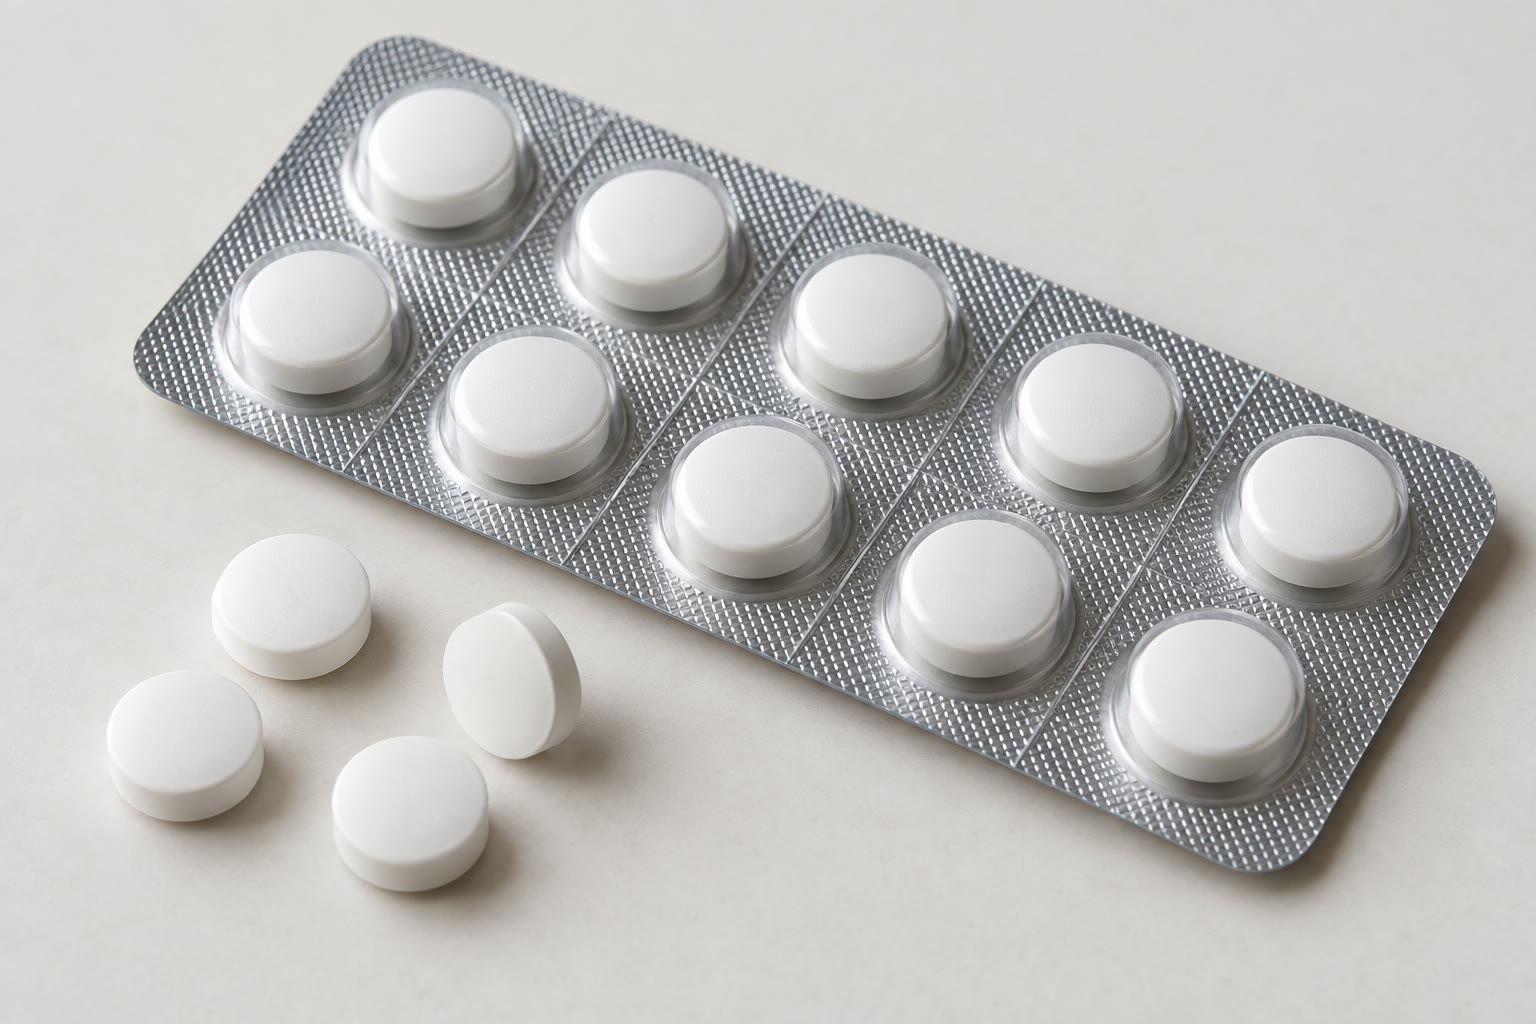
\includegraphics[width=0.45\linewidth]{images/book1/ai/g10-aspirin-tablets.jpg}

{\small Aspirinetabletten: elke tablet bevat een afgewogen massa van de
\omterm{def:g6:pure-substances-and-mixtures:pure-substance}{zuivere stof}, gemengd met een bindmiddel.}
\end{omfigure}

\section{Oefeningen}


\begin{exercise}[$\star$]\label{exo:g10:synthesis-yield:1}
Een \omterm{def:g10:synthesis-yield:synthesis}{synthese} kon hoogstens \qty{5.0}{g} product geven; er wordt
\qty{4.2}{g} zuiver, droog product verkregen. Bereken het \omterm{def:g10:synthesis-yield:yield}{rendement}.
\end{exercise}

\begin{exercise}[$\star$]\label{exo:g10:synthesis-yield:2}
Zet deze stappen van een \omterm{def:g10:synthesis-yield:synthesis}{synthese} in de goede volgorde: het smeltpunt
meten; \omterm{def:g10:synthesis-yield:reflux}{verwarmen onder terugvloeiing}; \omterm{def:g10:synthesis-yield:recrystallisation}{herkristallisatie}; \omterm{def:g10:synthesis-yield:vacuum-filtration}{vacuümfiltratie}
van het \omterm{def:g10:synthesis-yield:synthesis}{ruwe product}; de \omterm{def:g7:chemical-reactions:reactant}{beginstoffen} afwegen.
\end{exercise}

\begin{exercise}[$\star$]\label{exo:g10:synthesis-yield:3}
Waarom wordt bij een opstelling met terugvloeiing het koelwater onderaan
in de koeler geleid? Waarom blijft de bovenkant van de koeler open?
\end{exercise}

\begin{exercise}[$\star$]\label{exo:g10:synthesis-yield:4}
Welke twee eigenschappen moet een \omterm{def:g6:solutions-and-solubility:solute}{oplosmiddel} hebben om een product te
herkristalliseren? Waar komen de verontreinigingen terecht?
\end{exercise}

\begin{exercise}[$\star$]\label{exo:g10:synthesis-yield:5}
% ledger: mp:aspirin
Een monster gesynthetiseerde aspirine smelt tussen \qty{124}{\celsius} en
\qty{130}{\celsius}. Zuivere aspirine smelt bij ongeveer
\qty{135}{\celsius}. Is het monster zuiver? Wat moet er gebeuren?
\end{exercise}

\begin{exercise}[$\star\star$]\label{exo:g10:synthesis-yield:6}
Er reageert \qty{2.00}{g} salicylzuur met ethaanzuuranhydride in
overmaat; er wordt \qty{2.03}{g} zuivere, droge aspirine verkregen.
Bereken de maximale massa aspirine en het \omterm{def:g10:synthesis-yield:yield}{rendement}.
\end{exercise}

\begin{exercise}[$\star\star$]\label{exo:g10:synthesis-yield:7}
Een leerling weegt haar aspirine terwijl die nog nat is en vindt een
\omterm{def:g10:synthesis-yield:yield}{rendement} van \qty{104}{\percent}. Verklaar dit. Zou het wegen van het
\omterm{def:g10:synthesis-yield:synthesis}{ruwe product}, ongezuiverd maar droog, een \omterm{def:g10:synthesis-yield:yield}{rendement} geven dat te hoog of
te laag is vergeleken met het echte \omterm{def:g10:synthesis-yield:yield}{rendement}?
\end{exercise}

\begin{exercise}[$\star\star$]\label{exo:g10:synthesis-yield:8}
Noem twee voordelen van een \omterm{def:g10:synthesis-yield:vacuum-filtration}{vacuümfiltratie} boven een gewone filtratie
door een papieren kegel, om kristallen te verzamelen.
\end{exercise}

\begin{exercise}[$\star\star$]\label{exo:g10:synthesis-yield:9}
Op een DLC-plaatje heeft het front van het \omterm{def:g10:chemical-species:tlc}{eluens} \qty{5.0}{cm}
afgelegd. De vlek van een gesynthetiseerd product heeft \qty{3.1}{cm}
afgelegd, die van zuivere aspirine \qty{3.1}{cm}, die van salicylzuur
\qty{2.2}{cm}. Bereken de drie \omterm{def:g10:chemical-species:retention-factor}{retentiefactoren}. Wat kun je over het
product concluderen?
\end{exercise}

\begin{exercise}[$\star\star$]\label{exo:g10:synthesis-yield:10}
De \omterm{def:g6:solutions-and-solubility:solubility}{oplosbaarheid} van een product in twee \omterm{def:g6:solutions-and-solubility:solute}{oplosmiddelen} is:
\begin{center}
\begin{tabular}{lcc}
\hline
\omterm{def:g6:solutions-and-solubility:solute}{oplosmiddel} & koud (\qty{20}{\celsius}) & heet (bij het kookpunt) \\
\hline
A & \qty{2}{g/L} & \qty{150}{g/L} \\
B & \qty{80}{g/L} & \qty{120}{g/L} \\
\hline
\end{tabular}
\end{center}
Welk \omterm{def:g6:solutions-and-solubility:solute}{oplosmiddel} is beter voor een \omterm{def:g10:synthesis-yield:recrystallisation}{herkristallisatie}? Hoeveel heet
\omterm{def:g6:solutions-and-solubility:solute}{oplosmiddel} is er ongeveer nodig voor \qty{3.0}{g} \omterm{def:g10:synthesis-yield:synthesis}{ruw product}, en
hoeveel blijft er hoogstens opgelost als het koud is?
\end{exercise}

\begin{exercise}[$\star\star$]\label{exo:g10:synthesis-yield:11}
Waarom is de rondbodemkolf van een opstelling met terugvloeiing nooit
meer dan half vol? Waarom worden er kooksteentjes toegevoegd?
\end{exercise}

\begin{exercise}[$\star\star\star$]\label{exo:g10:synthesis-yield:12}
Een geneesmiddel wordt gemaakt in twee stappen, met \omterm{def:g10:synthesis-yield:yield}{rendementen} van
\qty{80}{\percent} en \qty{70}{\percent}. Wat is het totale \omterm{def:g10:synthesis-yield:yield}{rendement}?
Wat zou het zijn bij drie stappen van elk \qty{90}{\percent}? Waarom
proberen scheikundigen geneesmiddelen in zo weinig mogelijk stappen te
maken?
\end{exercise}

\begin{exercise}[$\star\star\star$]\label{exo:g10:synthesis-yield:13}
% ledger: sol:aspirin-25
Aspirine lost in water op tot ongeveer \qty{3.3}{g/L} bij
\qty{25}{\celsius}. Kristallen worden gewassen met \qty{50}{mL} water van
die temperatuur. Hoeveel aspirine kan er hoogstens verloren gaan? Waarom
wordt het waswater eerst in ijs gekoeld?
\end{exercise}

\begin{exercise}[$\star\star\star$]\label{exo:g10:synthesis-yield:14}
Er wordt \qty{2.76}{g} salicylzuur gemengd met \qty{0.0500}{mol}
ethaanzuuranhydride. Na de reactie wordt er water toegevoegd, dat het
overtollige anhydride vernietigt: \ce{C4H6O3 + H2O -> 2C2H4O2}.
\begin{enumerate}
  \item Vul de \omterm{def:g10:reaction-progress-table:extent}{voortgangstabel} van de \omterm{def:g10:synthesis-yield:synthesis}{synthese} in; hoeveel anhydride
        blijft er over?
  \item Hoeveel ethaanzuur is er aan het eind in totaal aanwezig?
\end{enumerate}
\end{exercise}

\begin{exercise}[$\star\star\star$]\label{exo:g10:synthesis-yield:15}
Een fabriek moet \qty{1.00}{t} aspirine maken, met een totaal \omterm{def:g10:synthesis-yield:yield}{rendement}
van \qty{85}{\percent} vanaf salicylzuur. Hoeveel salicylzuur moet ze
kopen?
\end{exercise}

\section{Probleem: Aspirine maken}

\begin{problem}[{Weekendprobleem --- van drie gram salicylzuur tot een
potje zuivere aspirine: wat is het rendement?}]
\label{pb:g10:synthesis-yield:1}
% ledger: rho:acetic-anhydride, mp:aspirin, mp:salicylic, sol:aspirin-25, aw:C, aw:H, aw:O
Een klas maakt aspirine. In de kolf: \qty{3.0}{g} salicylzuur en
\qty{6.0}{mL} ethaanzuuranhydride, met een dichtheid van
\qty{1.08}{g/mL}, en een paar druppels zuur; het \omterm{def:g6:pure-substances-and-mixtures:mixture}{mengsel} wordt verwarmd
onder terugvloeiing. Het \omterm{def:g10:synthesis-yield:synthesis}{ruwe product} dat met \omterm{def:g10:synthesis-yield:vacuum-filtration}{vacuümfiltratie} verzameld
wordt, weegt nat \qty{3.6}{g} en droog \qty{3.3}{g}. Na \omterm{def:g10:synthesis-yield:recrystallisation}{herkristallisatie}
en drogen blijft er \qty{2.7}{g} witte kristallen over.

\medskip
\noindent\textbf{Deel I --- De reactie.}
\begin{enumerate}
  \item Controleer dat de vergelijking
        \ce{C7H6O3 + C4H6O3 -> C9H8O4 + C2H4O2} klopt.
  \item Bereken de \omterm{def:g10:the-mole:molar-mass}{molaire massa's} van salicylzuur,
        ethaanzuuranhydride, aspirine en ethaanzuur.
  \item Noem de \omterm{def:g7:chemical-reactions:reactant}{beginstoffen}, het gewenste product en het bijproduct.
  \item Waarom wordt het \omterm{def:g6:pure-substances-and-mixtures:mixture}{mengsel} verwarmd onder terugvloeiing en niet in
        een open kolf?
\end{enumerate}

\medskip
\noindent\textbf{Deel II --- De maximale massa.}
\begin{enumerate}[resume]
  \item Bereken de beginhoeveelheid salicylzuur.
  \item Bereken de massa, en daarna de hoeveelheid, ethaanzuuranhydride.
  \item Vul de \omterm{def:g10:reaction-progress-table:extent}{voortgangstabel} in. Welke \omterm{def:g7:chemical-reactions:reactant}{beginstof} is beperkend? Geef
        $x_{\max}$.
  \item Leid daaruit de maximale massa aspirine af.
  \item Waarom wordt het anhydride in overmaat toegevoegd, en niet het
        salicylzuur?
\end{enumerate}

\medskip
\noindent\textbf{Deel III --- Isoleren en zuiveren.}
\begin{enumerate}[resume]
  \item Waarom kun je de natte massa, \qty{3.6}{g}, niet gebruiken om een
        \omterm{def:g10:synthesis-yield:yield}{rendement} te berekenen?
  \item Bereken het \omterm{def:g10:synthesis-yield:yield}{rendement} aan droog \omterm{def:g10:synthesis-yield:synthesis}{ruw product}.
  \item Waarom verlaagt de \omterm{def:g10:synthesis-yield:recrystallisation}{herkristallisatie} de massa?
  \item De kristallen werden gewassen met \qty{30}{mL} water van
        \qty{25}{\celsius}, waarin aspirine \omterm{def:g2:mixing-and-dissolving:dissolve}{oplost} tot ongeveer
        \qty{3.3}{g/L}. Hoeveel kon er op die manier hoogstens verloren
        gaan?
  \item Bereken het \omterm{def:g10:synthesis-yield:yield}{rendement} aan zuiver product.
\end{enumerate}

\medskip
\noindent\textbf{Deel IV --- Het product controleren.}
\begin{enumerate}[resume]
  \item De geherkristalliseerde kristallen smelten scherp bij
        \qty{135}{\celsius}. Wat laat dat zien?
  \item Het \omterm{def:g10:synthesis-yield:synthesis}{ruwe product} smolt tussen \qty{120}{\celsius} en
        \qty{131}{\celsius}. Wat laat dat zien?
  \item Op een DLC-plaatje geeft het \omterm{def:g10:synthesis-yield:synthesis}{ruwe product} twee vlekken, een op
        de hoogte van zuivere aspirine en een op de hoogte van
        salicylzuur; het geherkristalliseerde product geeft één vlek, op
        de hoogte van aspirine. Trek je conclusie.
  \item De vlek van het geherkristalliseerde product heeft \qty{3.1}{cm}
        afgelegd en het front van het \omterm{def:g10:chemical-species:tlc}{eluens} \qty{5.0}{cm}. Bereken de
        \omterm{def:g10:chemical-species:retention-factor}{retentiefactor}.
  \item In welk deel van het werk, de reactie of de \omterm{def:g10:synthesis-yield:recrystallisation}{herkristallisatie}, ging
        meer aspirine verloren?
  \item Geef het eindantwoord: wat is het \omterm{def:g10:synthesis-yield:yield}{rendement} van de \omterm{def:g10:synthesis-yield:synthesis}{synthese}?
\end{enumerate}
\end{problem}
